\section{Rotary encoder}
\begin{figure}[H]
    \centering
    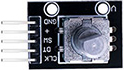
\includegraphics[angle=0, keepaspectratio=true, scale=1, width=200px, height=200px]{images/rotary.jpg}
    %\caption{Caption}
\end{figure}
\subsection*{Description}
This module is different from a potentiometer in that a rotary encoder has full rotation without limits. A rotary encoder module can tell the direction in which it was rotated and by how much.
\subsection*{Pin mapping}
This pin mapping corresponds to the pins from left to right with the module pins facing towards you.
\begin{table}[H]
    \centering
    \begin{tabular}{|c|c|c|c|c|}
    \hline
    Index &Label &Type &Name &Description\\ \hline
    0 &GND &Ground &GND &\\ \hline
    1 &+ &Source voltage &$V+$ &Module source voltage ($5V$)\\ \hline
    2 &SW &Digital input &D0 &Pushbutton switch\\ \hline
    3 &DT & & &Rotary phase B\\ \hline
    4 &CLK & & &Rotary phase A\\ \hline
    \end{tabular}
    %\caption{Caption}
    %\label{tab:my_label}
\end{table}
\subsection*{Operation}
The operation of this module is best explained at \href{https://lastminuteengineers.com/rotary-encoder-arduino-tutorial}{https://lastminuteengineers.com/rotary-encoder-arduino-tutorial}.
\subsection*{Code}
Refer to listing \ref{python_rotaryEncoder}.
%\lstinputlisting[caption=test]{laser.py}we